% ----------------------- TODO ---------------------------
% Diese Daten müssen pro Blatt angepasst werden:
\newcommand{\NUMBER}{5}
\newcommand{\EXERCISES}{5}
% Diese Daten müssen einmalig pro Vorlesung angepasst werden:
\newcommand{\COURSE}{Grundlagen der Digitaltechnik}
\newcommand{\TOPIC}{Anzeigen}
\newcommand{\DATE}{20.05.2022}
% ----------------------- TODO ---------------------------

\documentclass[a4paper]{scrartcl}

\usepackage[utf8]{inputenc}
\usepackage[ngerman]{babel}
\usepackage{amsmath}
\usepackage{amssymb}
\usepackage{fancyhdr}
\usepackage{color}
\usepackage{graphicx}
\usepackage{lastpage}
\usepackage{listings}
\usepackage{tikz}
\usepackage{pdflscape}
\usepackage{subfigure}
\usepackage{float}
\usepackage{polynom}
\usepackage{hyperref}
\usepackage{tabularx}
\usepackage{forloop}
\usepackage{geometry}
\usepackage{listings}
\usepackage{fancybox}
\usepackage{tikz}
\usepackage{algpseudocode,algorithm,algorithmicx}

%Definiere Let-Command für algorithmen
\newcommand*\Let[2]{\State #1 $\gets$ #2}

\input kvmacros

%Größe der Ränder setzen
\geometry{a4paper,left=3cm, right=3cm, top=3cm, bottom=3cm}

%Kopf- und Fußzeile
\pagestyle {fancy}
\fancyhead[L]{\COURSE}
\fancyhead[R]{\DATE}

\fancyfoot[L]{}
\fancyfoot[C]{}
\fancyfoot[R]{Seite \thepage /\pageref*{LastPage}}
\setlength{\parindent}{0pt}

%Formatierung der Überschrift, hier nichts ändern
\def\header#1#2{
  \begin{center}
    {\Large Labor #1: \TOPIC}\\
    {(Datum #2)}
  \end{center}
}


\begin{document}


\header{Nr. \NUMBER}{\DATE}


\section*{Aufgabe 1: Die 7-Segmentanzeige}
\begin{figure}[h]
  \centering
  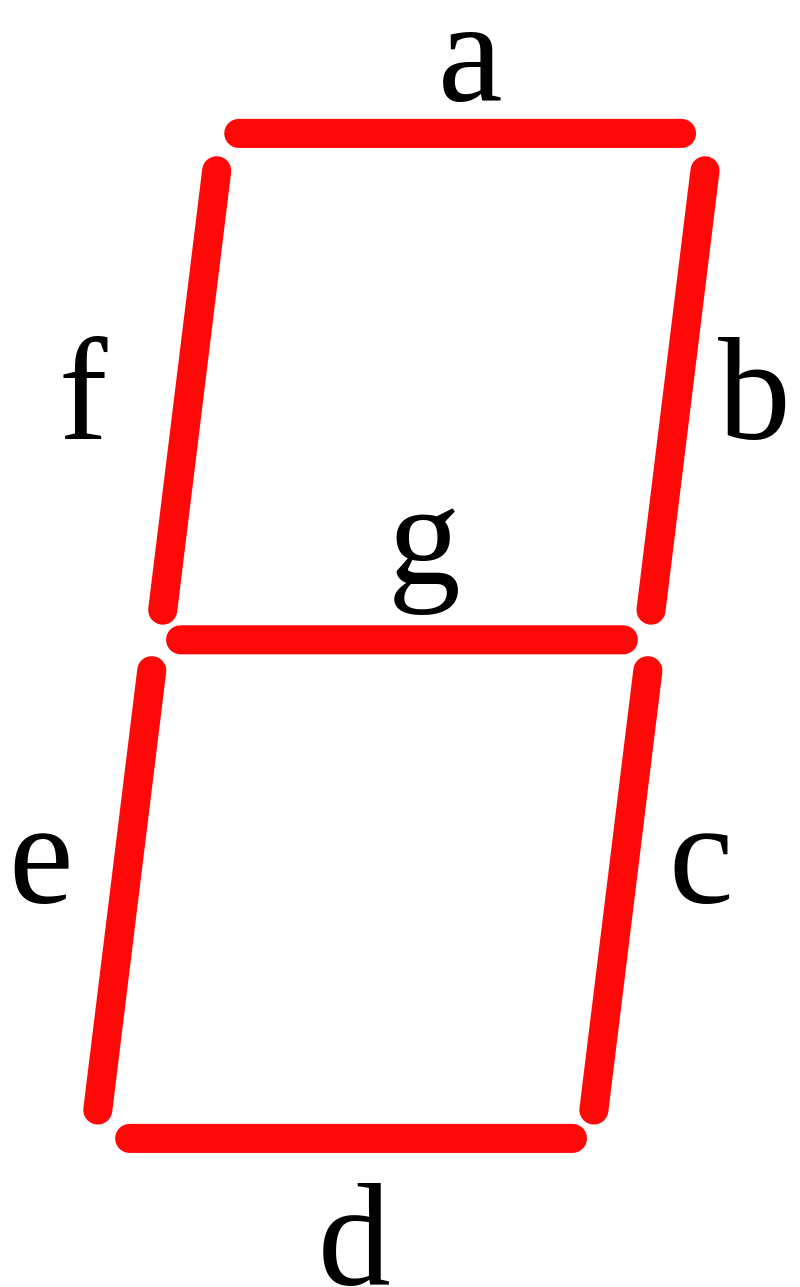
\includegraphics[width=3cm]{7segment.png}
  \caption{7-Segementanzeige}
\end{figure}
Das Bild zeigt eine 7-Segmentanzeige. Diese hat bestimmt jeder in irgendeinem Gerät schon ein mal gesehen. Die 7-Segmentanzeige funktioniert so, dass
jedes der Segemente über ein eigenes Signal an und ausgeschalten werden kann (A-G ist jeweils ein Signal). Vgl. hierzu auch das Bauteil \textit{7-Segment Display} in der Input/Output
Bibliothek von Logisim.
Für unsere Zwecke sollen mit der 7-Segmentanzeige Zahlen dargestellt werden.\\

Für den Umgang mit diesen Anzeigen kann zur einfacheren Benutzung der BCD-Code (Binary Coded Decimal) benutzt werden. Im BCD-Code werden die Zahlen 0-9 jeweils mit 4 Bit codiert.
Eine zweite Stelle (10er) wird dann wieder mit 4-Bit codiert (vgl. auch Tabelle).
\begin{table}[h]
  \centering
  \begin{tabular}{l|l|l|l}
    Bin. & Dez. & $BCD_{High}$ & $BCD_{Low}$ \\ \hline
    \texttt{0000} & 0 & \texttt{0000} & \texttt{0000}\\ 
    \texttt{0001} & 1 & \texttt{0000} & \texttt{0001}\\ 
    \texttt{0010} & 2 & \texttt{0000} & \texttt{0010}\\ 
    \texttt{0011} & 3 & \texttt{0000} & \texttt{0011}\\ 
    \texttt{0100} & 4 & \texttt{0000} & \texttt{0100}\\ 
    \texttt{0101} & 5 & \texttt{0000} & \texttt{0101}\\ 
    \texttt{0110} & 6 & \texttt{0000} & \texttt{0110}\\ 
    \texttt{0111} & 7 & \texttt{0000} & \texttt{0111}\\ 
    \texttt{1000} & 8 & \texttt{0000} & \texttt{1000}\\ 
    \texttt{1001} & 9 & \texttt{0000} & \texttt{1001}\\     
    \texttt{1010} & 10 & \texttt{0001} & \texttt{0000}\\     
    \texttt{1011} & 11 & \texttt{0001} & \texttt{0001}\\     
  \end{tabular}
  \caption{BCD-Code}
\end{table}

Eine BCD Tetrade (4-Bits) kann nun verwendet um eine einzelne 7-Segmentanzeige anzusteuern. Dies kann natürlich nicht direkt geschehen, 
da jedes Segment ein eigenes Signal besitzt

\subsection*{a) BCD 2 7Seg}
Erstelle in Logisim einen ``BCD to 7 Segments'' Converter. Das Subsystem soll 4 Bits als Input haben und die Ausgänge A-G für die 7-Segmentanzeige.
Die folgende Tabelle kann als Wahrheitstabelle benutzt werden.\\


\textbf{Mögliches Vorgehen:}
\begin{itemize}
  \item Gehe für jedes Segment die Zahlen 0-9 durch und ermittle, ob das Segment an oder aus sein muss
  \item Trage für ``an'' eine 1 in die Tabelle, für ``aus'' eine 0
  \item Ermittle für jedes Segement aus der Wahrheitstabelle mit dem KV-Diagram die disjunktive Minimalform
  \item Implementiere diese mit Hilfe von Logisim
\end{itemize}

\begin{table}[h]
  \centering
  \begin{tabular}{l|l|l|l|l|l|l|l|l}
    Dez. & Bin. & A & B & C & D & E & F & G \\ \hline
    0 & \texttt{0000}&&&&&&&\\ 
    1 & \texttt{0001}&&&&&&&\\ 
    2 & \texttt{0010}&&&&&&&\\ 
    3 & \texttt{0011}&&&&&&&\\ 
    4 & \texttt{0100}&&&&&&&\\ 
    5 & \texttt{0101}&&&&&&&\\ 
    6 & \texttt{0110}&&&&&&&\\ 
    7 & \texttt{0111}&&&&&&&\\ 
    8 & \texttt{1000}&&&&&&&\\ 
    9 & \texttt{1001}&&&&&&&\\     
  \end{tabular}
\end{table}

\begin{table}[h]
  \centering
  \Huge
  \begin{tabular}{c|wc{1em}|wc{1em}|wc{1em}|wc{1em}|c}%wc{1em}|wc{1em}|wc{1em}|wc{1em}|c} 
    & \multicolumn{2}{c|}{$x_0$}     &\multicolumn{2}{c}{$\overline{x_0}$}& \\ \cline{1-6}
    $x_1$ &&&&& $\overline{x_3}$ \\\cline{2-6}
    &&&&& $x_3$            \\\cline{1-5}
    $\overline{x_1}$   &&&&&                  \\\cline{2-6}
    &&&&& $\overline{x_3}$ \\\cline{2-6}
    &$\overline{x_2}$&\multicolumn{2}{c|}{$x_2$}&$\overline{x_2}$&\\
  \end{tabular}
\end{table}

Nach der Implementierung soll die Schaltung mit einem 7-Segments Display getestet werden.


\subsection*{b) Binary 2 BCD}
Jede BCD-Tetrade kann direkt mit einer Anzeige verbunden werden. Typischerweise liegen  Zahlen in digitalen Schaltungen aber
Binär-Codiert und nicht direkt im BCD-Code vor. Um daher die Möglichkeit zu haben
mehrere (Dezimal-)Stellen anzuzeigen, braucht man einen Binary to BCD Converter.

Um Binary in BCD umzuwandeln kann der ``Double Dabble'' Algorithmus benutzt werden.\\
Mehr Infos dazu hier:\\
\href{https://www.youtube.com/watch?v=eXIfZ1yKFlA}{https://www.youtube.com/watch?v=eXIfZ1yKFlA}\\
\href{https://en.wikipedia.org/wiki/Double_dabble}{https://en.wikipedia.org/wiki/Double\_dabble}\\


Da diese Implementierung ein bisschen zu weit führt verwenden für die Übung einfach den Binary to BCD
Converter, welcher Logisim anbietet: in ``BFH mega functions''.\\
{\tiny
  (Hier gibt es übrigens auch einen BCD  to 7Seg Converter, welcher gerade in mühevoller Handarbeit erstellt wurde ;-D)
}

\subsection*{c) 4-Stellige Anzeige}
Erstelle mit Hilfe des selbst designten BCD  to 7Seg Converter, des Binary to BCD Converters aus der Library und vier 7-Segmentanzeigen eine Schaltung,
welche einen 10-Bit Input als vier stellige Integer-Zahl darstellt.

\section*{Aufgabe 2: Das Voltmeter}
Ein Voltmeter besitzt ein 12-Bit ADC. Dieser ADC codiert Spannungen zwischen 0 und 4,095 Volt mit diesen 12 Bits binär.
Zusätzlich besitzt das Voltmeter am Eingang einen Spannungsteiler, welcher durch einen Drehknauf eingestellt werden kann.
Es gibt die Stufen:
\begin{itemize}
  \item keine Teilung
  \item Teilung auf 1/2
  \item Teilung auf 1/10
  \item Teilung auf 1/20
  \item Teilung auf 1/100
\end{itemize} 
Das folgende Bild zeigt einen exemplarischen Schaltplan der Eingangsstufe.
Diese Eingangsstufe gibt folgende Signale an die weitere Schaltung aus (nicht im Schaltplan eingezeichnet):
\begin{itemize}
  \item D11..D0: die 12 Datenbits
  \item $T_1, T_{2}, T_{10}, T_{20}, T_{100}$: High wenn jeweilige Teilung aktiv
\end{itemize}

\textbf{Hinweis:}\\
Die 7-Segment Displays haben neben den Signalen für die 7-Segmentanzeige auch ein Signal für einen Dezimalpunkt. 

\subsection*{a) Entwurf}
Baue mit den Angaben zum Voltmeter und den
Resultaten aus Aufgabe 1 eine Schaltung,
welche die Daten der Eingangsstufe korrekt als 4-stellige Dezimalzahl darstellt.\\



\begin{figure}
  \centering
  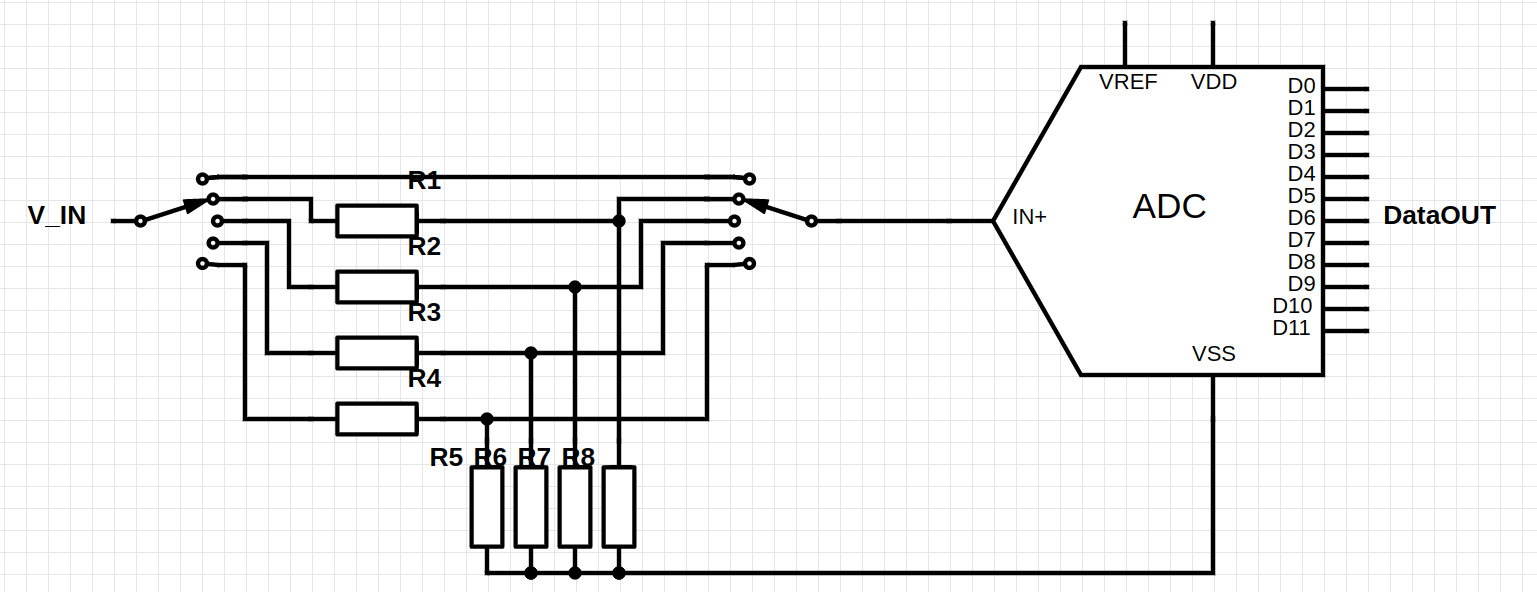
\includegraphics[width=12cm]{Voltmeter.png}
  \caption{Exemplarisch: die Eingangsschaltung (die beiden Schalter bewegen sich synchron)}
\end{figure}

\newpage
\textbf{Hinweise:}
\begin{itemize}
  \item Die Ausganssignale der Eingangsstufe sind die Eingänge der Schaltung
  \item Mit den Ausgängen der Schaltung sollen die 7 Segment Displays (einschließlich Dezimalpunkt) angesteuert werden.
  \item Wie hängt 1-Bit des ADCs mit der Eingangsspannung am ADC zusammen?
  \item Bedenke die Displays sollen immer die tatsächliche Eingangsspannung vor dem Spannungsteiler anzeigen.
  \item Mache dir bewusst, was der ADC ``sieht'', wenn eine Spannung vorher schon geteilt wird. Und wie groß diese Spannung ``wirklich'' ist.
  \item Wenn ein ADC über- oder untersteuert wird, wird der Max.- bzw. Minwert ausgegeben.
  \item Durch die Teiler-Signale muss der Dezimalpunkt (Punkt=Komma) korrekt gesetzt werden.
  \begin{itemize}
    \item 1.023
    \item 10.23
    \item 102.3
  \end{itemize}
  \item Für eine bestimmte Teilereinstellung soll der Dezimalpunkt unabhängig vom Wert immer an der gleichen Stelle sein
  \item Nutze einen Multiplizierer von Logisim wo nötig
\end{itemize}

\subsection*{b) Test}
Auf Moodle gibt es eine Schaltung, welche die Eingangsschaltung des Voltmeters simulieren soll (InputCircuitVoltmeter). Diese hat einen $V_{IN}$ Eingang, welcher
den Analogeingang des Voltmeters simulieren soll (in echt ist es lediglich ein 32-Bit Floating Point). Wenn an ihn ein 32-Bit breiter Pin angeschlossen und dieser
auf ``Float'' umgestellt wird, kann dort eine Kommazahl als Eingang eingestellt werden. Diese soll die Eingangsspannung an den Klemmen des Voltmeters darstellen.
Der Ausgang der Schaltung ist der 12-Bit breite ADC-Ausgang.
Die Eingänge T1 - T100 stellen das Teilerverhältnis dar. Hier sollte 
lediglich immer nur ein Eingang ``high'' sein. Bei mehreren ``high'' Eingangsignalen gewinnt das höchste Teilerverhältnis.\\
Teste mit dieser Schaltung, die Schaltung aus Aufgabenteil a). \\

\textbf{Fragen:}\\
Was ist die höchste Spannung die das Voltmeter anzeigen kann?\\
Warum gibt es die Teilereinstellungen?\\
Was ist der Vorteil einer niedrigen Teilereinstellung?\\
Was der einer hohen?\\

\textbf{Hinweis:}\\
Falls es mit der Verschaltung Probleme gibt vgl. das folgende Bild:
\begin{figure}[h!]
  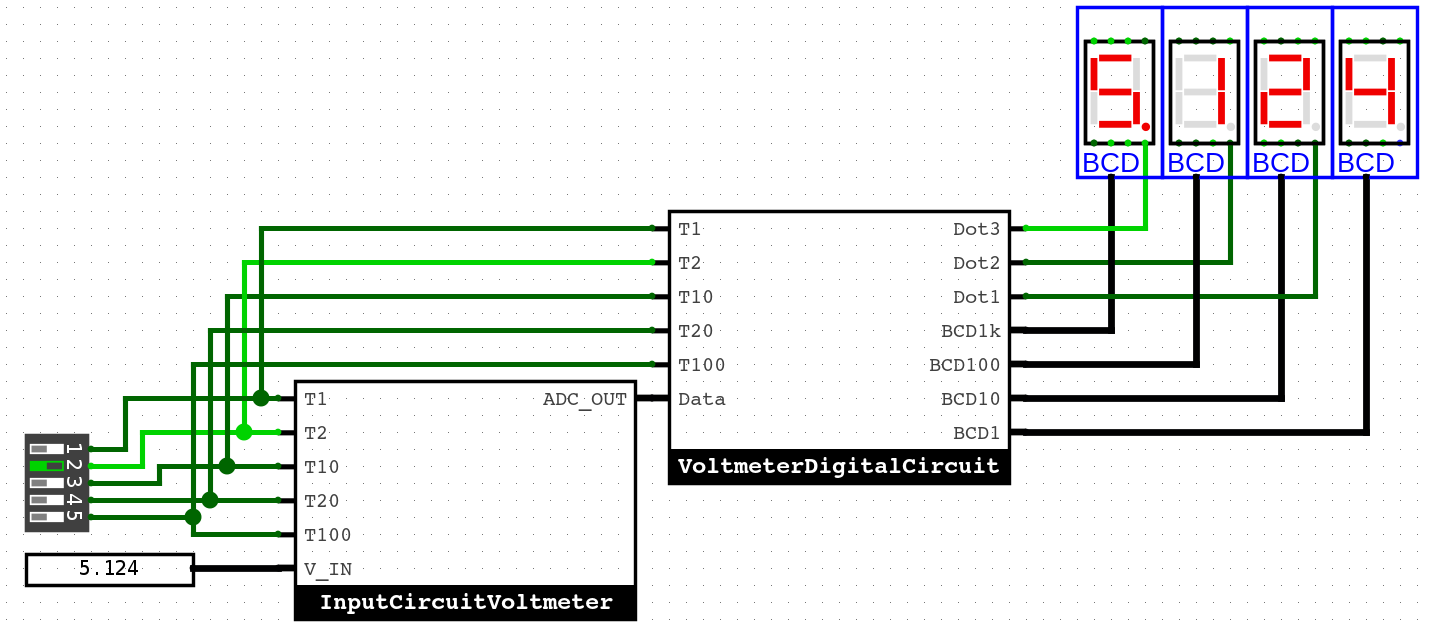
\includegraphics[width=\textwidth]{Voltmeter_Dig.png}
  \caption{Beispielverschaltung: Voltmeter}
\end{figure}




\section*{Aufgabe 3: Digital Uhr}
Baue mit den 7-Segement Displays eine Digitaluhr, welche Stunden, Minuten und Sekunden anzeigt. Der Eingang soll ein 1 Hz Clk-Signal sein.\\

\textbf{Hinweise:}
\begin{itemize}
  \item Es werden mehrere Zähler benötigt (Stunden, Minuten, Sekunden)
  \item Diese Zähler müssen sich bei einem bestimmten Grenzwert ``resetten''. 
  \item Es ist möglich bei einem Logisim-Counter ein Max-Wert einzustellen (Feature muss nicht benutzt werden)
  \item Der Maxwert-Ausgang eines Zählers kann als Eingang des nächsten benutzt werden.
\end{itemize}

\end{document}
%%% Local Variables:
%%% mode: latex
%%% TeX-master: t
%%% End: